\section{Eksperimen}
\label{sec:eksperimen}

\subsection{Pengujian Gerakan}

\begin{figure} [ht]
  \centering
  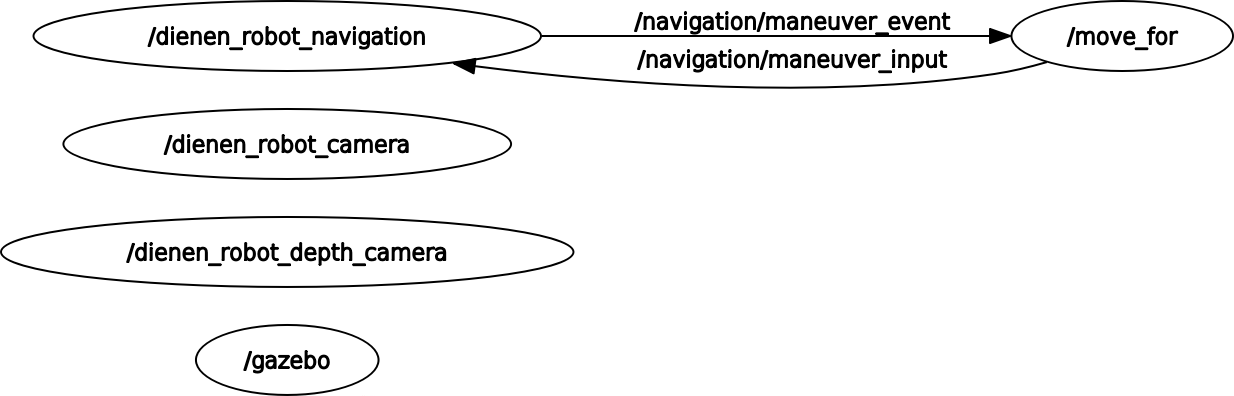
\includegraphics[scale=0.25]{gambar/nodeujigeraksimulasi.png}
  \caption{Skema \emph{node} pengujian gerakan di simulasi.}
  \label{fig:nodeujigeraksimulasi}
\end{figure}

\begin{figure} [ht]
  \centering
  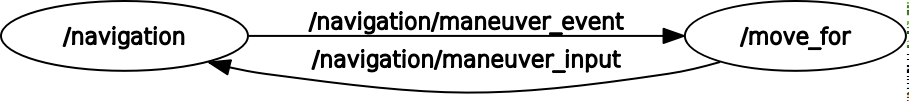
\includegraphics[scale=0.3]{gambar/nodeujigerakfisik.png}
  \caption{Skema \emph{node} pengujian gerakan pada robot fisik.}
  \label{fig:nodeujigerakfisik}
\end{figure}

Pengujian gerakan dilakukan dengan menjalankan \emph{node} \lstinline{move_for} sebagai \emph{node behavior} yang akan memerintahkan robot untuk bergerak dengan kecepatan tertentu selama kurun waktu tertentu.
Seperti yang terlihat pada Gambar \ref{fig:nodeujigeraksimulasi}, di simulasi, \emph{node} \lstinline{move_for} akan terhubung dengan \emph{node} \lstinline{dienen_robot_navigation} untuk mengatur kecepatan dari robot yang ada di simulasi menggunakan \emph{topic} \lstinline{/navigation/maneuver_input}.
Sedangkan untuk pengujian di dunia nyata, seperti yang terlihat pada Gambar \ref{fig:nodeujigerakfisik}, peran dari \emph{node} \lstinline{dienen_robot_navigation} yang mengatur navigasi pada robot virtual akan digantikan oleh \emph{node} \lstinline{navigation} yang mengatur navigasi yang ada pada robot fisik.

\begin{table}
  \caption{Hasil uji gerakan linier di simulasi selama 10 detik.}
  \label{tab:hasilujiliniersimulasi}
  \centering
  \begin{tabular}{cc|cc|cc}
    \toprule
    \multicolumn{2}{c|}{Kecepatan} &
    \multicolumn{2}{|c|}{Posisi di Simulasi} &
    \multicolumn{2}{|c}{Posisi Odometri} \\
    \midrule
    x (m/min) & y (m/min) & x (m) & y (m) & x(m)  & y(m) \\
    \midrule
    40        & 0         & 5.2   & 0.0   & 5.2   & 0.0 \\
    60        & 0         & 7.9   & 0.0   & 7.9   & 0.0 \\
    -40       & 0         & -5.2  & 0.0   & -5.2  & 0.0 \\
    0         & 40        & 0.0   & 5.4   & 0.0   & 5.4 \\
    0         & -40       & 0.0   & -5.3  & 0.0   & -5.3 \\
    40        & 20        & 5.0   & 3.0   & 5.0   & 3.0 \\
    -20       & 40        & -2.9  & 5.5   & -2.9  & 5.5 \\
    \bottomrule
  \end{tabular}
\end{table}

\begin{table}
  \caption{Hasil uji gerakan sudut di simulasi selama 10 detik.}
  \label{tab:hasilujisudutsimulasi}
  \centering
  \begin{tabular}{c|c|c}
    \toprule
    Kecepatan   & Orientasi di Simulasi & Orientasi Odometri \\
    \midrule
    z (rad/min) & z (deg)               & z (deg) \\
    \midrule
    40          & 39.0                  & 39.0 \\
    120         & 118.7                 & 118.7 \\
    -40         & -39.2                 & -39.2 \\
    -120        & -117.1                & -117.1 \\
    \bottomrule
  \end{tabular}
\end{table}

Pengujian gerakan terbagi menjadi dua bagian, pengujian gerakan linier dan pengujian gerakan sudut, masing-masing diujikan selama 10 detik pada robot virtual di lingkungan simulasi dan pada robot fisik di dunia nyata.
Seperti yang terlihat pada Tabel \ref{tab:hasilujiliniersimulasi} dan Tabel \ref{tab:hasilujisudutsimulasi}, posisi dan orientasi odometri yang diterima robot memiliki nilai yang sama dengan posisi dan orientasi model robot di simulasi.
Hal ini terjadi karena nilai odometri yang dikirimkan oleh node \lstinline{dienen_robot_navigation} adalah nilai yang sama dengan transformasi model robot di simulasi.

\begin{table}
  \caption{Hasil uji gerakan linier pada robot fisik selama 10 detik.}
  \label{tab:hasilujilinierdunianyata}
  \centering
  \begin{tabular}{cc|cc|cc}
    \toprule
    \multicolumn{2}{c|}{Kecepatan} &
    \multicolumn{2}{|c|}{Posisi di Dunia Nyata} &
    \multicolumn{2}{|c}{Posisi Odometri} \\
    \midrule
    x (m/min) & y (m/min) & x (m) & y (m) & x(m)  & y(m) \\
    \midrule
    40        & 0         & 5.1   & -0.1  & 5.2   & 0.1 \\
    60        & 0         & 8.1   & 0.1   & 7.9   & 0.0 \\
    -40       & 0         & -5.3  & 0.1   & -5.2  & 0.1 \\
    0         & 40        & 0.0   & 5.4   & 0.1   & 5.2 \\
    0         & -40       & 0.2   & -5.1  & -0.1  & -5.5 \\
    40        & 20        & 5.2   & 3.1   & 5.3   & 3.1 \\
    -20       & 40        & -3.1  & 5.3   & -2.9  & 5.3 \\
    \bottomrule
  \end{tabular}
\end{table}

\begin{table}
  \caption{Hasil uji gerakan sudut pada robot fisik selama 10 detik.}
  \label{tab:hasilujisudutdunianyata}
  \centering
  \begin{tabular}{c|c|c}
    \toprule
    Kecepatan   & Orientasi di Dunia Nyata  & Orientasi Odometri \\
    \midrule
    z (rad/min) & z (deg)                   & z (deg) \\
    \midrule
    40          & 41.0                      & 39.6 \\
    120         & 120.0                     & 119.3 \\
    -40         & -40.0                     & -39.6 \\
    -120        & -119.0                    & -116.2 \\
    \bottomrule
  \end{tabular}
\end{table}

Berbeda dengan pengujian di lingkungan simulasi, pengujian di dunia nyata memiliki hasil yang berbeda antara pengukuran langsung dengan nilai odometri yang diterima oleh robot.
Seperti yang terlihat pada Tabel \ref{tab:hasilujilinierdunianyata} dan Tabel \ref{tab:hasilujisudutdunianyata}, terdapat perbedaan antara keduanya yang disebabkan oleh ketidakakuratan yang ada pada sensor yang digunakan untuk mendapatkan nilai posisi dan orientasi.
Walaupun begitu, terlepas dari adanya perbedaan tingkat akurasi, dengan menggunakan \emph{node behavior} yang sama, robot tergolong mampu melakukan perintah gerakan yang sesuai ketika diujikan di simulasi maupun di dunia nyata.
